\documentclass[oneside,12pt]{memoir}

\usepackage{amsthm}
\usepackage{amsmath}
\usepackage{amssymb}
\usepackage{mathtools}
\usepackage{enumitem}
\usepackage{hyperref}
\usepackage{tikz}
\usetikzlibrary{arrows.meta}
\usetikzlibrary{decorations.markings}

\hypersetup{colorlinks=true,urlcolor=blue}

\newcommand{\bb}{\mathbb}
\newcommand{\mc}{\mathcal}
\newcommand{\ms}{\mathscr}

\makeoddhead{myheadings}{Math 381}{Discrete Mathematical Modeling}{\thepage}
\pagestyle{myheadings}

\setlist[enumerate,2]{label = (\alph*)}

\begin{document}

\begin{center}
\textbf{\large Homework 4} \\
\emph{Due Friday, January 26}
\end{center}

\begin{enumerate}[leftmargin=*]

\item Winston, Problem 2(a), page 472
\item Winston, Problem 16, page 431
\item A \emph{clique} of an undirected graph is a set $C$ of vertices such that for any two vertices $u$, $v$ in $C$, there is an edge between $u$ and $v$. For example, in the below graph, $\{1,2,4,6\}$ is a clique of size 4, and there are no cliques of larger size. Thus $\{1,2,4,6\}$ is a clique of maximum size.
	\begin{center}
	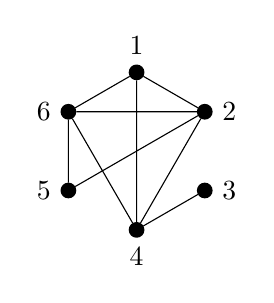
\begin{tikzpicture}[vertex/.style={circle, fill, minimum size=2mm, inner sep=0mm, outer sep=0mm}]
		\node[vertex,label=above:1] at (90:1) (1) {};
		\node[vertex,label=right:2] at (30:1) (2) {};
		\node[vertex,label=right:3] at (330:1) (3) {};
		\node[vertex,label=below:4] at (270:1) (4) {};
		\node[vertex,label=left:5] at (210:1) (5) {};
		\node[vertex,label=left:6] at (150:1) (6) {};
		\draw (1)--(2)--(5) (6)--(1)--(4)--(2)--(6) (3)--(4)--(6)--(5);
	\end{tikzpicture}
	\end{center}
	Given an undirected graph $G$, formulate an integer program which finds a clique of $G$ of maximum size. (If there are multiple largest cliques, the IP only needs to find one of them.) The info you are given is the set of vertices and the set of edges of the graph, and your IP will depend on this information. You do not need to code your IP.
\item Consider the LP relaxation of your IP from problem 4. Show that for the below graph, the LP relaxation gives a different optimal value than the IP.
	\begin{center}
	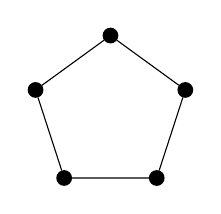
\begin{tikzpicture}[vertex/.style={circle, fill, minimum size=2mm, inner sep=0mm, outer sep=0mm}]
		\node[vertex] at (90:1) (1) {};
		\node[vertex] at (18:1) (2) {};
		\node[vertex] at (306:1) (3) {};
		\node[vertex] at (234:1) (4) {};
		\node[vertex] at (162:1) (5) {};
		\draw (1)--(2)--(3)--(4)--(5)--(1);
	\end{tikzpicture}
	\end{center}
\end{enumerate}
\end{document}